\section{Method}\label{method}

In this section the different components of the project are described. It gives an account of how the query completion module has been implemented. A frontend has also been implemented to provide a better environment for testing and demoing. Lastly, the section contains details on how the implementation was tested and what requirements the implementation should fulfill. 

\subsection{Implementation}

As previously mentioned, Apache Solr has built-in support for free text search. It is contained in the class org.apache.solr.spelling.suggest.Suggester and is configured in the file solrconfig.xml.. In order to implement our query suggestion, a new class, SuggesterMK2, has been implemented which piggybacks on the existing functionality of the original Suggester class.
[http://wiki.apache.org/solr/Suggester]

The SuggesterMK2 implementation attempts to be a drop-in replacement for the Suggester class. Notable exceptions to this general rule include:
\begin{itemize}

\item The |SuggesterMK2| uses the query parameter |spellcheck.q| instead of the parameter |q|
\item The |SuggesterMK2| uses a custom field in |solrconfig.xml| called |delegate| instead of the field called |field|.
\end{itemize}

The rationale for these seemingly arbitrary decisions will be stated explicitly in the coming sections of this report.

\subsubsection{Delegation}

The |SuggesterMK2| implementation uses the delegation pattern |http://en.wikipedia.org/wiki/Delegation_pattern| in order to reuse the original suggester implementation as much as possible. Reusing the original Suggester class means that we can use the original implementations query suggestion implementation, as well as its loading and reloading implementations, all of which we can assume work and would be distinctly tricky to implement from scratch.

\begin{figure}[h!]
    \centering
    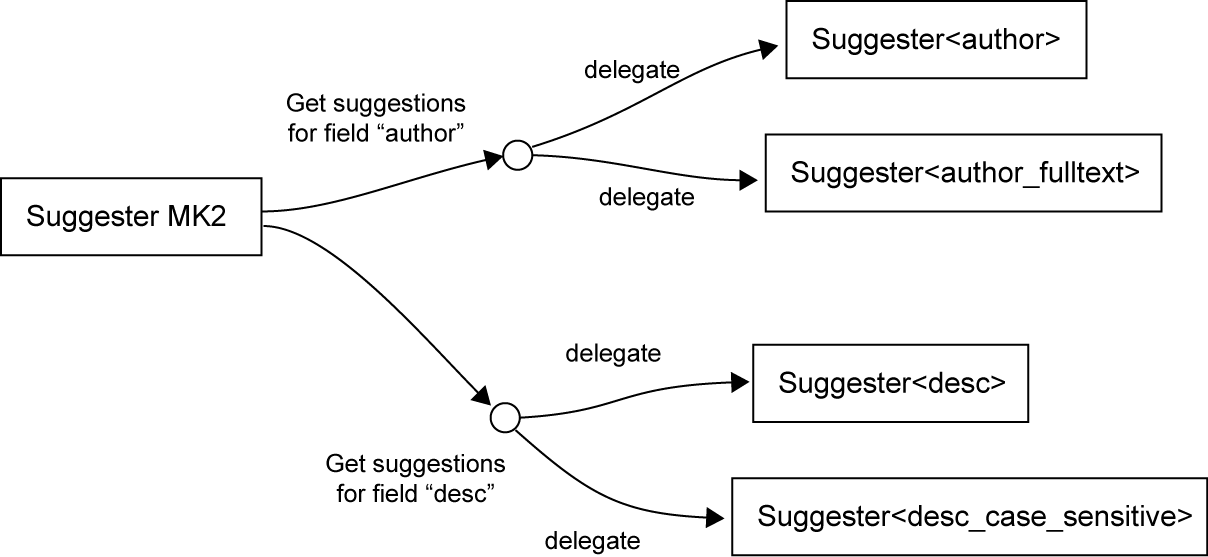
\includegraphics[width=0.8\textwidth]{img/delegation.png}
    \caption{Representation of the delegation done by SuggesterMK2}
    \label{fig:delegation}
\end{figure}

Let us for instance say that we configure the system to give suggestions for the field |author| using the contents from the fields |author| and |author_exact| the first of which being tokenized on whitespace, and the second being untokenized. All we have to do then, using delegation, is to construct a |Suggester| object for each field |author| and |author_exact|, query each of these, and then combine the results, merging results as needed if the results overlap. In our implementation, configuring the suggester to return results as in the diagram can be done by adding the following to the suggester configuration in |solrconfig.xml|.

\begin{verbatim}
<lst name=''delegate''>
  <str name=''targetField''>author</str>
  <str name=''sourceField''>author</str>
  <str name=''sourceField''>author_fulltext</str>
</lst>
\end{verbatim}

The fields we use for contents do not need to include the target field – we can use the contents from entirely different fields to use as suggestions. For a sample use case where this might be desired, consider what would happen if the target field were 4-gram tokenized: a word like ''parallelize'' would then be split up into the tokens ''para'', ''aral'', ''rall'', ''alle'', and so on, none of which we want to give as query suggestions. We would then want to draw suggestions from some other field where the contents are tokenized as words instead.

The |SuggesterMK2| implementation also gives query suggestions consisting of the field names it is configured to give suggestions for. For instance, the example configuration in figure \ref{delegation} the |SuggesterMK2| would give |author:”| as a query suggestion when the user types |aut|.

For the full configuration of the suggester in solrconfig.xml, see Appendix.
For the implementation of the SuggesterMK2, see [https://github.com/actinium/ir14-project.git]

\subsubsection{Order of results}

The results of a query are returned in a given order. Field names are given priority over field contents, while field contents and standard results are both sorted based on number of occurrences. For example of this see section \ref{results}.

\subsubsection{Frontend}

A simple frontend has been implemented to act as a tool for debugging and demoing the project. It uses JSON requests and responses to interact with the ''suggest'' and ''select'' features of the Solr server.

\subsubsection{Testing}

Testing was primarily done using the Solr Admin console and our own frontend.
In the early stages of development, test data provided by Solr was used. This was replaced with a larger test set of documents containing fields for names, party affiliation and quotes from members of Swedish parliament later on. A number of queries were used to test that the suggester performed as expected. These queries, as well as the result of the tests for the final version, can be found in the following section. 
